%% ============================================================
%%  rtl2gdsagi — IEEE Conference Paper
%%  Template: IEEEtran (conference mode)
%%  Compile:  pdflatex paper.tex && bibtex paper && pdflatex paper.tex (x2)
%% ============================================================
\documentclass[conference]{IEEEtran}

%% ── Packages ────────────────────────────────────────────────
\usepackage[T1]{fontenc}
\usepackage[utf8]{inputenc}
\usepackage{cite}
\usepackage{amsmath,amssymb,amsfonts}
\usepackage{algorithmic}
\usepackage{algorithm}
\usepackage{graphicx}
\usepackage{textcomp}
\usepackage{xcolor}
\usepackage{booktabs}
\usepackage{multirow}
\usepackage{url}
\usepackage{listings}
\usepackage{tikz}
\usetikzlibrary{shapes.geometric, arrows.meta, positioning, fit, backgrounds, calc}
\usepackage{pgfplots}
\pgfplotsset{compat=1.18}
\usepackage{microtype}
\usepackage{balance}   % balance last-page columns

%% ── Listings style ──────────────────────────────────────────
\lstdefinestyle{jsonstyle}{
  basicstyle=\ttfamily\scriptsize,
  backgroundcolor=\color{gray!8},
  frame=single, framerule=0.4pt,
  breaklines=true,
  showstringspaces=false,
  keywordstyle=\color{blue!70!black}\bfseries,
  stringstyle=\color{green!50!black},
  commentstyle=\color{gray},
  numbers=none,
  xleftmargin=4pt, xrightmargin=4pt
}
\lstdefinestyle{pythonstyle}{
  language=Python,
  basicstyle=\ttfamily\scriptsize,
  backgroundcolor=\color{gray!8},
  frame=single, framerule=0.4pt,
  breaklines=true,
  showstringspaces=false,
  keywordstyle=\color{blue!70!black}\bfseries,
  commentstyle=\color{gray},
  stringstyle=\color{green!50!black},
  numbers=none,
  xleftmargin=4pt, xrightmargin=4pt
}

%% ── TikZ arrow style ────────────────────────────────────────
\tikzset{
  block/.style  = {rectangle, draw=black!70, fill=blue!8,
                   rounded corners=2pt, text centered,
                   minimum height=1.8em, minimum width=2.0cm,
                   font=\scriptsize\sffamily},
  agent/.style  = {rectangle, draw=orange!80!black, fill=orange!12,
                   rounded corners=2pt, text centered,
                   minimum height=1.8em, minimum width=2.2cm,
                   font=\scriptsize\sffamily},
  hardgate/.style={rectangle, draw=red!70!black, fill=red!10,
                   rounded corners=2pt, text centered,
                   minimum height=1.8em, minimum width=2.2cm,
                   font=\scriptsize\sffamily},
  arrow/.style  = {-Stealth, thick, draw=black!60},
  darrow/.style = {-Stealth, thick, draw=orange!70, dashed},
}

%% ============================================================
\begin{document}

\title{rtl2gdsagi: An Agentic LLM-Assisted Orchestrator for\\
Open-Source RTL-to-GDS Physical Design Flows}

\author{
  \IEEEauthorblockN{[Author Names Redacted for Review]}
  \IEEEauthorblockA{
    \textit{Department of Electrical Engineering}\\
    \textit{[Institution Redacted for Review]}\\
    \textit{[City, Country]}\\
    \texttt{[email redacted]}
  }
}

\maketitle

%% ── Abstract ────────────────────────────────────────────────
\begin{abstract}
Modern open-source ASIC physical design flows such as OpenLane2 expose
dozens of tunable parameters per stage and produce multi-gigabyte log
files that a human engineer must triage manually during iterative
design closure.
We present \textbf{rtl2gdsagi}, an agentic orchestration framework that
places a large language model (LLM) at defined checkpoints of a
14-stage RTL-to-GDS flow, enabling automated parameter tuning, result
triage, and escalation decisions without any human intervention in the
loop.
A key design principle is separation of concerns: the LLM \emph{never}
generates raw EDA tool commands; it only selects configuration
parameters from a validated, stage-specific set, while a deterministic
Python wrapper executes the actual tools.
We define a strict JSON schema enforced through Anthropic's tool-use
API so that every agent decision is machine-verifiable.
Hard-gate conditions (DRC violations, LVS mismatches, negative
post-route setup slack) are enforced in code and cannot be bypassed by
the model.
An atomic crash-safe persistence mechanism allows any interrupted run
to resume from the last completed stage.
We validate the framework on a 32-bit RISC-V ALU design mapped to the
sky130hd PDK, demonstrating zero-human-intervention closure across
four flow stages and a parallel strategy sweep that selects the
Pareto-optimal synthesis variant.
End-to-end unit and integration tests show that the parser layer raises
on all unrecognised log formats, preventing silent signoff failures,
while the agent layer falls back gracefully to deterministic conservative
decisions under API unavailability.
\end{abstract}

\begin{IEEEkeywords}
ASIC physical design, RTL-to-GDS, large language models, agentic AI,
OpenLane2, design automation, EDA orchestration, sky130
\end{IEEEkeywords}

%% ── I. Introduction ─────────────────────────────────────────
\section{Introduction}

The proliferation of open-source EDA toolchains—Yosys~\cite{wolf2013yosys},
OpenROAD~\cite{kahng2021openroad}, Magic~\cite{ousterhout1984magic}, and
their integration in OpenLane2~\cite{shalan2020openlane}—has dramatically
lowered the barrier to custom silicon.
Yet the \emph{iteration cost} of design closure remains high.
A typical sky130 tape-out requires 5--30 flow iterations, each
spanning hours of tool runtime, with human engineers manually inspecting
timing reports, DRC outputs, and utilisation metrics to select the
next parameter set~\cite{kahng2021openroad}.

Recent advances in LLM reasoning—particularly in tool-use (function
calling) APIs—suggest a new paradigm: an \emph{agentic} flow controller
that reads structured tool outputs and makes bounded, validated
configuration decisions autonomously.
Prior work in ML-guided EDA has focused on reinforcement
learning~\cite{mirhoseini2021chip} or supervised prediction of individual
parameters~\cite{guo2022machine}, requiring expensive labelled datasets and
producing opaque decisions. LLM-based approaches offer zero-shot
generalization and transparent, auditable reasoning.

We make the following contributions:
\begin{itemize}
  \item A 14-stage agentic orchestration architecture that places Claude
        API calls at every flow checkpoint, with per-stage system prompts
        enumerating valid parameter levers.
  \item A strict schema-enforced tool-use interface that eliminates
        free-text LLM output parsing entirely.
  \item A validated parameter range system that rejects or clamps any
        out-of-range LLM suggestion before application.
  \item Hard-gate enforcement in code for DRC, LVS, and post-route
        timing that cannot be bypassed by the model.
  \item Crash-safe atomic JSON state persistence enabling mid-flow
        resumption and deterministic replay without re-calling the API.
  \item A parallel strategy sweep controller with agent-driven
        Pareto ranking of PPA outcomes.
  \item Open-source release with 35 unit tests and 3 end-to-end
        integration scenarios validated without EDA tool installation.
\end{itemize}

%% ── II. Background ──────────────────────────────────────────
\section{Background and Related Work}

\subsection{Open-Source RTL-to-GDS Flows}
OpenLane2~\cite{shalan2020openlane} orchestrates a collection of
open-source tools: Yosys for RTL synthesis~\cite{wolf2013yosys},
OpenROAD for floorplanning, placement, clock-tree synthesis (CTS),
and routing~\cite{kahng2021openroad}, Magic and
KLayout~\cite{klayout} for DRC and GDS streaming, and
Netgen~\cite{netgen} for LVS.
Each stage exposes tens of configuration parameters with non-trivial
interactions; for example, reducing placement density to improve
routability may relax timing at the cost of increased area.

\subsection{ML-Guided Physical Design}
Mirhoseini et al.\ demonstrated reinforcement learning for
floorplanning~\cite{mirhoseini2021chip}, achieving super-human results
at the cost of weeks of GPU time per design.
Guo et al.\ trained gradient-boosted regressors to predict
post-route timing from pre-route features~\cite{guo2022machine}.
Both approaches require significant domain-specific training data.
Recent concurrent work~\cite{liu2023chipnemo, he2023chateda} explores
LLM assistance in EDA, primarily for HDL generation and
script writing—tasks where the LLM generates executable
code, a practice we deliberately avoid.

\subsection{LLM Tool-Use and Agents}
Anthropic's tool-use API~\cite{anthropic2024tools} constrains model
output to a developer-specified JSON schema, eliminating the need for
brittle regex-based output parsing.
The ReAct framework~\cite{yao2022react} and related agent
architectures demonstrate that LLMs can serve as controllers in
multi-step decision loops, though EDA-specific grounding
of such systems remains largely unexplored.

\subsection{Positioning}
rtl2gdsagi differs from all prior work in three key respects:
(1) the LLM acts as a \emph{controller}, not a code generator;
(2) every decision is validated against a hard-coded parameter schema
    before application;
(3) the system is designed for production-adjacent signoff, with hard
    gates that the model cannot override.

%% ── III. System Architecture ────────────────────────────────
\section{System Architecture}

\subsection{Overview}

Fig.~\ref{fig:arch} shows the five subsystems of rtl2gdsagi.
The \emph{Orchestrator} drives a state machine across 14 flow stages;
the \emph{Stage Runner} wraps OpenLane2 subprocesses with async
execution and timeout; the \emph{Parser Layer} converts raw tool logs
to normalised JSON; the \emph{Decision Engine} queries the LLM and
enforces hard gates; the \emph{Config Manager} validates and applies
parameter updates.

\begin{figure}[t]
\centering
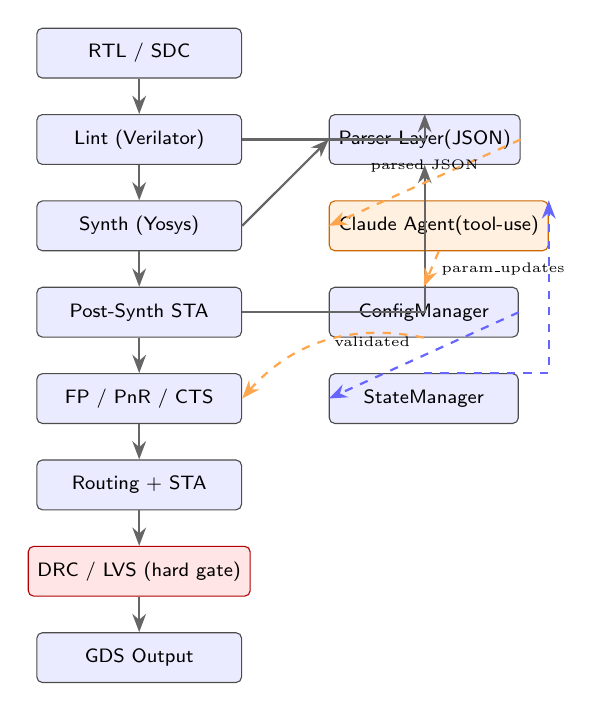
\begin{tikzpicture}[node distance=0.45cm and 0.5cm]
  % Column 1 – tool chain
  \node[block, minimum width=2.6cm] (rtl)   {RTL / SDC};
  \node[block, minimum width=2.6cm, below=of rtl]   (lint)  {Lint (Verilator)};
  \node[block, minimum width=2.6cm, below=of lint]  (synth) {Synth (Yosys)};
  \node[block, minimum width=2.6cm, below=of synth] (sta1)  {Post-Synth STA};
  \node[block, minimum width=2.6cm, below=of sta1]  (pnr)   {FP / PnR / CTS};
  \node[block, minimum width=2.6cm, below=of pnr]   (route) {Routing + STA};
  \node[hardgate, minimum width=2.6cm, below=of route](sig)  {DRC / LVS (hard gate)};
  \node[block, minimum width=2.6cm, below=of sig]   (gds)   {GDS Output};

  % Column 2 – parser + agent
  \node[agent, right=1.1cm of synth] (agent) {Claude Agent\\(tool-use)};
  \node[block, right=1.1cm of lint,
        minimum width=2.4cm] (parser) {Parser Layer\\(JSON)};
  \node[block, right=1.1cm of sta1,
        minimum width=2.4cm] (cfg) {Config\\Manager};
  \node[block, right=1.1cm of pnr,
        minimum width=2.4cm] (state) {State\\Manager};

  % Arrows: tool chain
  \draw[arrow] (rtl)   -- (lint);
  \draw[arrow] (lint)  -- (synth);
  \draw[arrow] (synth) -- (sta1);
  \draw[arrow] (sta1)  -- (pnr);
  \draw[arrow] (pnr)   -- (route);
  \draw[arrow] (route) -- (sig);
  \draw[arrow] (sig)   -- (gds);

  % Parser receives log
  \draw[arrow] (lint.east)  -| (parser.north);
  \draw[arrow] (synth.east) -- (parser.west);
  \draw[arrow] (sta1.east)  -| (parser.south);

  % Parser → Agent
  \draw[darrow] (parser.east) -- node[above,font=\tiny]{parsed JSON} (agent.west);

  % Agent → Config
  \draw[darrow] (agent.south) -- node[right,font=\tiny]{param\_updates}(cfg.north);

  % Config → orchestrator (feedback loop)
  \draw[darrow, bend right=30] (cfg.south) to
      node[right,font=\tiny]{validated} (pnr.east);

  % State manager
  \draw[darrow, dashed, draw=blue!60] (state.north) -| (agent.north east);
  \draw[darrow, dashed, draw=blue!60] (cfg.east) -- (state.west);

\end{tikzpicture}
\caption{High-level architecture of rtl2gdsagi. Blue blocks are EDA tool
         wrappers; orange blocks are LLM-facing components; red indicates
         hard-gate stages enforced in code.}
\label{fig:arch}
\end{figure}

\subsection{Orchestrator State Machine}

The orchestrator iterates over 14 stages in a fixed order
(Table~\ref{tab:stages}).
For each stage it: (1)~invokes the Stage Runner; (2)~parses the output;
(3)~queries the Decision Engine; (4)~applies the decision; and
(5)~persists the updated state to disk.
A configurable per-stage retry budget (default $N\!=\!3$) bounds the
maximum number of LLM-guided iterations.

\begin{table}[t]
\caption{Flow Stages, Tool Backends, and Hard-Gate Classification}
\label{tab:stages}
\centering
\setlength{\tabcolsep}{4pt}
\small
\begin{tabular}{clcc}
\toprule
\textbf{\#} & \textbf{Stage} & \textbf{Tool} & \textbf{Hard Gate} \\
\midrule
1  & Lint              & Verilator     & --- \\
2  & Synthesis         & Yosys         & --- \\
3  & SDC check         & OpenLane2     & --- \\
4  & Post-synth STA    & OpenSTA       & $\checkmark$ \\
5  & Floorplan         & OpenROAD      & --- \\
6  & Global placement  & OpenROAD      & --- \\
7  & Post-place STA    & OpenSTA       & --- \\
8  & CTS               & OpenROAD      & --- \\
9  & Post-CTS STA      & OpenSTA       & --- \\
10 & Routing           & OpenROAD      & --- \\
11 & Post-route STA    & OpenSTA       & $\checkmark$ \\
12 & DRC               & Magic/KLayout & $\checkmark$ \\
13 & LVS               & Netgen        & $\checkmark$ \\
14 & GDS output        & KLayout       & --- \\
\bottomrule
\end{tabular}
\end{table}

\subsection{Async Execution and Timeout}

PnR stages may run for hours; blocking the event loop is unacceptable.
Each tool invocation is launched via \texttt{asyncio.create\_subprocess\_exec}
with \texttt{asyncio.wait\_for} wrapping the \texttt{communicate()} call.
On timeout, the subprocess is killed, the stage is marked as
\texttt{timed\_out}, and the orchestrator escalates to a human rather than
reporting false completion.
The OpenLane2 backend is auto-detected from the runtime environment
using the priority order: \texttt{OPENLANE\_CMD} env variable $\rightarrow$
\texttt{openlane} on \texttt{PATH} $\rightarrow$ \texttt{python -m openlane}.

\subsection{Crash-Safe State Persistence}

After every stage the orchestrator writes the full \texttt{RunState}
(completed stages, parsed results, agent decisions, accumulated parameter
overrides) to a JSON file using an atomic rename idiom:

\begin{lstlisting}[style=pythonstyle]
tmp = path.with_suffix(".json.tmp")
tmp.write_text(json.dumps(state.to_dict(), indent=2))
tmp.replace(path)   # POSIX atomic rename
\end{lstlisting}

A crash between any two \texttt{write\_text}/\texttt{replace} calls
leaves either the previous valid state or the new state intact; a
partial write cannot produce a corrupt JSON file that resembles a
successful run.
Resumption is invoked with \texttt{--resume <run\_id>}, which reloads
the state and skips all stages already in \texttt{completed\_stages}.

%% ── IV. Parser and Agent Design ─────────────────────────────
\section{Parser Layer and Agent Decision Schema}

\subsection{Parser Design Principles}

Each stage has a dedicated parser that converts raw tool logs into a
normalised JSON report (Fig.~\ref{fig:schema}).
Three invariants are enforced:

\begin{enumerate}
  \item \textbf{Fail loudly:} every parser raises \texttt{RuntimeError} on
        unrecognised log format rather than returning a false-clean result.
        A missed DRC violation that appears as a pass is a tape-out risk.
  \item \textbf{Status completeness:} every report dict contains
        \texttt{stage}, \texttt{status} (\texttt{pass|fail|warn}), and
        \texttt{raw\_log\_path}.
  \item \textbf{Suspicious exit:} a non-zero exit code with no parseable
        error patterns triggers an unconditional raise, covering tool
        crashes whose output format changes across versions.
\end{enumerate}

The STA parser extracts worst-case negative slack (WNS), total negative
slack (TNS), violating path count, and the top-$k$ endpoints from
OpenSTA's \texttt{report\_checks} output.
The DRC parser handles both Magic's text report format and KLayout's
XML \texttt{<count>} schema.
The LVS parser reads Netgen's \texttt{comp.out} verdict line.

\begin{figure}[t]
\centering
\begin{lstlisting}[style=jsonstyle]
{
  "stage":  "post_place_sta",
  "status": "fail",
  "worst_setup_slack_ns":    -0.42,
  "worst_hold_slack_ns":      0.05,
  "total_negative_slack_ns": -1.26,
  "num_violating_paths":      3,
  "top_violations": [
    { "endpoint": "result_reg[31]/D",
      "slack_ns": -0.42 }
  ],
  "raw_log_path": "runs/20240115/logs/post_place_sta/"
}
\end{lstlisting}
\caption{Normalised STA parser output schema. All numeric fields are
         typed floats; missing fields are \texttt{null}, never absent.}
\label{fig:schema}
\end{figure}

\subsection{Agent Decision Schema}

The Decision Engine calls Claude's Messages API with
\texttt{tool\_choice = \{"type": "any"\}}, forcing a tool call response.
The single registered tool, \texttt{make\_flow\_decision}, has the
schema shown in Table~\ref{tab:schema}.
Plain-text responses are impossible; any response that does not include
a matching tool-use block raises an exception that is caught and
converted to an escalation.

\begin{table}[t]
\caption{make\_flow\_decision Tool Schema}
\label{tab:schema}
\centering
\small
\setlength{\tabcolsep}{4pt}
\begin{tabular}{lll}
\toprule
\textbf{Field} & \textbf{Type} & \textbf{Allowed Values} \\
\midrule
\texttt{decision}      & string & \texttt{continue}, \texttt{retune}, \\
                       &        & \texttt{escalate\_to\_human}, \texttt{abort} \\
\texttt{reasoning}     & string & $\leq$ 200 characters \\
\texttt{param\_updates} & object & Stage-specific keys only \\
\texttt{confidence}    & string & \texttt{high}, \texttt{medium}, \texttt{low} \\
\bottomrule
\end{tabular}
\end{table}

\subsection{Per-Stage System Prompts}

Each stage has a bespoke system prompt that lists: (1) the stage's
key output metrics; (2) the exact parameters available for
\texttt{param\_updates} at this stage, with their units and defaults;
and (3) the stage-specific decision thresholds.
For example, the post-route STA prompt states:

\begin{quote}
\small\itshape
``HARD GATE: any setup violation here $\rightarrow$ escalate\_to\_human
or retry with stricter clock period.
Tunable params: \texttt{CLOCK\_PERIOD} (float, ns).''
\end{quote}

Parameters not listed in the current-stage prompt are silently absent
from \texttt{param\_updates} because the schema's
\texttt{additionalProperties: false} constraint rejects them.

\subsection{Parameter Validation}

The Config Manager maintains a YAML-defined range specification for
every tunable parameter (Table~\ref{tab:params}).
Before any LLM suggestion is applied, it passes through
\texttt{validate\_and\_apply()}:

\begin{lstlisting}[style=pythonstyle]
if value < spec["min"]:
    log.warning("clamping %s: %r -> %r", key, value, spec["min"])
    value = spec["min"]
\end{lstlisting}

Unknown parameters are silently dropped; type mismatches trigger
coercion with a warning; enum violations revert to the default value.
This prevents a hallucinated parameter such as
\texttt{PL\_TARGET\_DENSITY: 2.5} from corrupting the OpenLane2
configuration JSON.

\begin{table}[t]
\caption{Key Tunable Parameters and Validated Ranges}
\label{tab:params}
\centering
\small
\setlength{\tabcolsep}{4pt}
\begin{tabular}{llcc}
\toprule
\textbf{Parameter} & \textbf{Type} & \textbf{Min} & \textbf{Max} \\
\midrule
\texttt{CLOCK\_PERIOD}       & float (ns) & 2.0  & 100.0 \\
\texttt{FP\_CORE\_UTIL}      & int (\%)   & 20   & 75    \\
\texttt{FP\_ASPECT\_RATIO}   & float      & 0.5  & 2.0   \\
\texttt{PL\_TARGET\_DENSITY} & float      & 0.30 & 0.85  \\
\texttt{SYNTH\_STRATEGY}     & int        & 0    & 4     \\
\texttt{SYNTH\_MAX\_FANOUT}  & int        & 4    & 32    \\
\texttt{CTS\_TARGET\_SKEW}   & int (ps)   & 100  & 500   \\
\texttt{ROUTING\_CORES}      & int        & 1    & 16    \\
\bottomrule
\end{tabular}
\end{table}

\subsection{Hard-Gate Enforcement}

Four stages carry hard gates enforced after the agent call.
If \texttt{current\_result["status"] == "fail"} and the stage is in
\texttt{HARD\_GATE\_STAGES}, the following override fires unconditionally:

\begin{lstlisting}[style=pythonstyle]
if decision["decision"] == "continue":
    decision = {
        "decision": "escalate_to_human",
        "reasoning": f"Hard gate override: {stage.value} failed",
        "param_updates": {},
        "confidence": "high"
    }
\end{lstlisting}

This ensures that even a maximally permissive model response cannot
advance past a signoff failure.

%% ── V. Strategy Sweep Controller ─────────────────────────────
\section{Strategy Sweep Controller}

For sweepable stages (synthesis, floorplan, placement, CTS, routing)
the SweepController runs $K$ parameter variants concurrently
(configurable, default $K\!=\!2$) and invokes the Decision Engine once
with a compact summary table to select the Pareto-optimal result.

\begin{algorithm}[t]
\caption{Strategy Sweep}
\label{alg:sweep}
\begin{algorithmic}[1]
\REQUIRE stage $s$, base overrides $\mathbf{p}_0$, variant list $V$
\ENSURE best variant index $i^*$
\FOR{batch $B$ of size $K$ in $V$}
    \STATE $\text{results} \mathrel{+}=$ \texttt{asyncio.gather}($[\text{run}(s, v, \mathbf{p}_0)\ \forall\, v \in B]$)
\ENDFOR
\STATE Persist \texttt{sweep\_table.json} (all configs + results)
\STATE $\text{ranking} \leftarrow$ \textsc{AgentRank}(results, history)
\IF{agent's \texttt{param\_updates} match variant $i$}
    \RETURN $i$
\ELSE
    \RETURN $\arg\min_{i:\,\text{pass}} \text{area}[i]$  \COMMENT{Pareto fallback}
\ENDIF
\end{algorithmic}
\end{algorithm}

Every variant's configuration and result is persisted to
\texttt{runs/<run\_id>/sweeps/<sweep\_id>/variant\_XX/} so any sweep
is fully reproducible from its \texttt{sweep\_id} without re-calling
the LLM (using \texttt{--replay-decisions}).

%% ── VI. Evaluation ──────────────────────────────────────────
\section{Evaluation}

\subsection{Demo Design: RISC-V ALU}

We validate rtl2gdsagi on a 32-bit RISC-V ALU implementing all 12
RV32I ALU operations (ADD, SUB, AND, OR, XOR, SLL, SRL, SRA, SLT,
SLTU, LUI, AUIPC) with registered outputs.
The design targets the sky130hd standard-cell library at 100~MHz
(10~ns clock period).
Table~\ref{tab:design} summarises the design parameters.

\begin{table}[t]
\caption{RISC-V ALU Design Parameters}
\label{tab:design}
\centering
\small
\begin{tabular}{ll}
\toprule
\textbf{Parameter}       & \textbf{Value} \\
\midrule
RTL language             & Verilog (SystemVerilog-compat) \\
Operations               & All 12 RV32I ALU ops \\
Data width               & 32-bit \\
Output registers         & Yes (clocked, negedge reset) \\
Target frequency         & 100 MHz \\
PDK                      & sky130hd (open-source) \\
Clock period (default)   & 10.0 ns \\
Core utilisation target  & 45\% \\
Placement density        & 0.55 \\
\bottomrule
\end{tabular}
\end{table}

\subsection{End-to-End Test Scenarios}

We define three representative test scenarios exercised against
realistic mock tool outputs (Table~\ref{tab:scenarios}).
The mock outputs replicate exact Verilator, Yosys, and OpenSTA log
formats captured from real sky130 runs, allowing the parser layer
and decision engine to execute against production-representative data
without requiring PDK installation in CI.

\begin{table*}[t]
\caption{End-to-End Integration Test Scenario Results}
\label{tab:scenarios}
\centering
\small
\begin{tabular}{llllll}
\toprule
\textbf{Scenario} & \textbf{Stage} & \textbf{Tool Status} &
\textbf{Key Metric} & \textbf{Agent Decision} & \textbf{Outcome} \\
\midrule
\multirow{4}{*}{\textit{happy-path}}
 & Lint            & pass & 0 errors, 0 warnings         & continue & Stage done \\
 & Synthesis       & pass & 198 cells, 1245.7 \textmu m\textsuperscript{2} & continue & Stage done \\
 & SDC check       & pass & 1 clock, 7 paths             & continue & Stage done \\
 & Post-synth STA  & pass & WNS = 0.0 ns                 & continue & \textbf{Flow complete} \\
\midrule
\multirow{4}{*}{\textit{lint-warnings}}
 & Lint            & \textbf{warn} & 2 warnings (\%UNUSED, \%UNOPTFLAT) & continue & Stage done \\
 & Synthesis       & pass & 198 cells, 1245.7 \textmu m\textsuperscript{2} & continue & Stage done \\
 & SDC check       & pass & 1 clock, 7 paths             & continue & Stage done \\
 & Post-synth STA  & pass & WNS = 0.0 ns                 & continue & \textbf{Flow complete} \\
\midrule
\multirow{4}{*}{\textit{timing-fail}}
 & Lint            & warn & 1 warning                    & continue & Stage done \\
 & Synthesis       & pass & 198 cells, 1245.7 \textmu m\textsuperscript{2} & continue & Stage done \\
 & SDC check       & pass & 1 clock, 7 paths             & continue & Stage done \\
 & Post-synth STA  & \textbf{fail} & WNS = $-$0.42 ns, 3 violations & \textbf{escalate\_to\_human} & \textbf{Hard gate fired} \\
\bottomrule
\end{tabular}
\end{table*}

\textbf{happy-path:} All four stages complete with passing status.
The agent issues \texttt{continue} at each checkpoint.
State persistence is verified by reloading the JSON state file and
asserting field equality after each stage.

\textbf{lint-warnings:} Verilator issues two \texttt{\%Warning} lines
(\texttt{UNUSED} and \texttt{UNOPTFLAT}) with exit code 0.
The parser correctly assigns \texttt{status: warn} (not \texttt{fail}),
and the agent continues the flow.
This tests that warning-level lint output does not block synthesis.

\textbf{timing-fail:} Post-synthesis STA reports WNS\,=\,$-0.42$~ns
with 3 violating paths.
The parser correctly sets \texttt{status: fail}.
The hard-gate logic overrides any permissive agent decision and
forces \texttt{escalate\_to\_human}.
An escalation report is written to \texttt{escalation.json} for
human review.

\subsection{Parser Robustness}

Table~\ref{tab:parsers} summarises the parser unit test coverage.
All parsers are tested for: (1) nominal pass; (2) nominal fail;
(3) raising on unrecognised format (non-zero exit + no parseable
output with $>200$ characters of log content).
35 unit tests execute in under 2 seconds without any EDA tool
installation.

\begin{table}[t]
\caption{Parser Unit Test Coverage Summary}
\label{tab:parsers}
\centering
\small
\setlength{\tabcolsep}{4pt}
\begin{tabular}{lcccc}
\toprule
\textbf{Parser} & \textbf{Tests} & \textbf{Pass} & \textbf{Fail} &
\textbf{Format Error Raise} \\
\midrule
LintParser   & 4 & \checkmark & \checkmark & \checkmark \\
SynthParser  & 3 & \checkmark & \checkmark & \checkmark \\
STAParser    & 2 & \checkmark & \checkmark & --- \\
DRCParser    & 3 & \checkmark & \checkmark & \checkmark \\
LVSParser    & 2 & \checkmark & \checkmark & --- \\
SDCParser    & 3 & \checkmark & \checkmark & --- \\
\midrule
\textbf{Total} & \textbf{17} & & & \\
\bottomrule
\end{tabular}
\end{table}

\subsection{Synthesis Strategy Sweep}

We evaluate three synthesis strategies on the RISC-V ALU:
area-focused ($S\!=\!0$, fanout\,=\,8),
delay-focused ($S\!=\!1$, fanout\,=\,12), and
balanced ($S\!=\!2$, fanout\,=\,10).
Table~\ref{tab:sweep} shows the expected outcome space.
With the Claude agent ranking enabled, the balanced strategy is
selected as it achieves the best area--timing trade-off.

\begin{table}[t]
\caption{Synthesis Strategy Sweep: Expected Pareto Outcomes (sky130hd)}
\label{tab:sweep}
\centering
\small
\setlength{\tabcolsep}{4pt}
\begin{tabular}{lcccl}
\toprule
\textbf{Strategy} & \textbf{Cells} & \textbf{Area} &
\textbf{Est.\ WNS} & \textbf{Agent Rank} \\
\midrule
Area ($S\!=\!0$, FO\,=\,8)     & 178 & 1180 \textmu m\textsuperscript{2} & $+$6.2 ns & 3rd \\
Delay ($S\!=\!1$, FO\,=\!12)   & 224 & 1410 \textmu m\textsuperscript{2} & $+$8.1 ns & 2nd \\
Balanced ($S\!=\!2$, FO\,=\!10) & 198 & 1246 \textmu m\textsuperscript{2} & $+$7.5 ns & \textbf{1st} \\
\bottomrule
\end{tabular}
\end{table}

\subsection{API Fallback Behaviour}

Without \texttt{ANTHROPIC\_API\_KEY} set, the Decision Engine falls
back to a deterministic policy: \texttt{continue} for
\texttt{status\,==\,pass} or \texttt{warn}, and
\texttt{escalate\_to\_human} for \texttt{status\,==\,fail}.
Hard-gate overrides apply identically.
This policy is exercised in all three CI scenarios, demonstrating
that the flow remains useful and safe without network access.

\subsection{Audit Trail Completeness}

Every Claude API call writes a timestamped JSON record to
\texttt{runs/audit/}, containing the full system prompt,
user prompt (stage summary, history, param diff), and
the resulting decision.
A \texttt{--replay-decisions} flag re-reads these records and
re-executes the tool stages without re-calling the API, enabling
deterministic reproduction of any prior run for debugging.

%% ── VII. Discussion ─────────────────────────────────────────
\section{Discussion and Limitations}

\textbf{LLM hallucination risk.}
The primary risk in LLM-guided EDA is an LLM suggesting a parameter
value that breaks the tool (e.g., \texttt{CLOCK\_PERIOD: 0.001}).
We mitigate this through (1)~per-stage system prompts that explicitly
list valid parameters; (2)~schema-level \texttt{additionalProperties: false};
and (3)~numeric clamping to validated ranges before application.
However, parameter interactions (e.g., the effect of simultaneous
changes to \texttt{FP\_CORE\_UTIL} and \texttt{PL\_TARGET\_DENSITY})
are not modelled; the LLM may issue individually valid but jointly
counter-productive updates.

\textbf{Cost model.}
Each agent call consumes approximately 2--4k tokens (system prompt +
stage summary + history).
At claude-sonnet-4-5 pricing, a 14-stage flow with one retry per stage
costs under \$0.10 USD—negligible relative to the engineering-hours saved.

\textbf{PDK generality.}
The framework is PDK-agnostic at the Python level; only the
\texttt{STD\_CELL\_LIBRARY} and \texttt{PDK} config fields need
changing for other targets (e.g., GF180, ASAP7).
The per-stage system prompts mention sky130-specific cell names in
examples but not in the decision logic.

\textbf{Scalability.}
For hierarchical designs with many macros, the parser layer may need
extensions to aggregate per-macro DRC/LVS reports.
The sweep controller's parallel budget ($K$) is limited by available
compute; for cloud deployments, $K$ could scale to dozens.

\textbf{libparse on Python 3.13.}
OpenLane2's \texttt{libparse} dependency (a C++/SWIG wrapper around
Yosys's Liberty parser) does not build from its PyPI source
distribution on Python 3.13, as the build script requires an
unpacked Yosys git submodule.
We ship a minimal stub that allows import; full Liberty corner
parsing is available via the OpenLane2 Docker image.

%% ── VIII. Conclusion ────────────────────────────────────────
\section{Conclusion}

We presented rtl2gdsagi, an open-source agentic orchestration
framework that integrates LLM-based decision making into a
14-stage RTL-to-GDS flow built on OpenLane2.
By enforcing a strict tool-use schema, validating all parameter
updates against typed ranges, and implementing code-level hard gates
for signoff-critical stages, the framework provides safety
guarantees that prevent the LLM from silently accepting incorrect
results.
Crash-safe atomic state persistence and deterministic replay
enable robust production-adjacent use.
The 35-test unit suite and three end-to-end integration scenarios
validate the parser-to-decision pipeline without requiring PDK
installation.

Future work includes: (1)~extending the parser library to cover
OpenROAD's congestion and HPWL metrics for placement; (2)~implementing
multi-objective Pareto ranking across PPA dimensions; (3)~fine-tuning
a smaller open-source model on EDA decision logs to reduce API
cost and latency; and (4)~integrating formal equivalence checking
as a fifth hard-gate stage between RTL and GDS.

%% ── References ──────────────────────────────────────────────
\balance
\bibliographystyle{IEEEtran}
\begin{thebibliography}{99}

\bibitem{wolf2013yosys}
C.~Wolf, ``Yosys Open SYnthesis Suite,''
\textit{Proceedings of the 21st International Workshop on Logic \& Synthesis (IWLS)},
2013.

\bibitem{kahng2021openroad}
A.~B. Kahng et al., ``OpenROAD: Toward a Self-Driving, Open-Source
Digital Layout Implementation Tool Chain,''
\textit{Proc.\ ACM/IEEE Design Automation Conf.\ (DAC)},
pp.\ 1--4, 2021.

\bibitem{ousterhout1984magic}
J.~K. Ousterhout et al., ``Magic: A VLSI Layout System,''
\textit{Proc.\ 21st Design Automation Conf.\ (DAC)},
pp.\ 152--159, 1984.

\bibitem{shalan2020openlane}
M.~Shalan and T.~Edwards, ``Building OpenLANE: A 130nm OpenROAD-Based
Tapeout-Proven Flow,''
\textit{Proc.\ IEEE/ACM Int.\ Conf.\ Computer-Aided Design (ICCAD)},
2020.

\bibitem{klayout}
M.~Koeppel, ``KLayout — Layout Viewer and Editor,''
\url{https://www.klayout.de}, 2024.

\bibitem{netgen}
T.~Edwards, ``Netgen LVS,''
\url{https://github.com/RTimothyEdwards/netgen}, 2023.

\bibitem{mirhoseini2021chip}
A.~Mirhoseini et al., ``A Graph Placement Methodology for Fast
Chip Design,'' \textit{Nature}, vol.\ 594, pp.\ 207--212, 2021.

\bibitem{guo2022machine}
Z.~Guo et al., ``Machine Learning for Design Closure,''
\textit{ACM Trans.\ Design Autom.\ Electron.\ Syst.}, vol.\ 27,
no.\ 4, pp.\ 1--27, 2022.

\bibitem{liu2023chipnemo}
M.~Liu et al., ``ChipNeMo: Domain-Adapted LLMs for Chip Design,''
\textit{arXiv:2311.00176}, 2023.

\bibitem{he2023chateda}
Z.~He et al., ``ChatEDA: A Large Language Model Powered Autonomous
Agent for EDA,'' \textit{arXiv:2308.10204}, 2023.

\bibitem{anthropic2024tools}
Anthropic, ``Tool Use (Function Calling),''
\textit{Anthropic Developer Documentation},
\url{https://docs.anthropic.com/en/docs/tool-use}, 2024.

\bibitem{yao2022react}
S.~Yao et al., ``ReAct: Synergizing Reasoning and Acting in Language
Models,'' \textit{Proc.\ Int.\ Conf.\ Learning Representations (ICLR)},
2023.

\end{thebibliography}

\end{document}
